% Introduce the webpage design (probably include code in appendix)
% Introduce preprocessing

% Include a folder on github repo to pretest code: 1) CoSE model; 2) AuDrA model; 3) DSI; 4) Mediation Analysis

\documentclass[../Proposal_Writing_Sample.tex]{subfiles}
% \documentclass[../Proposal_Ma_Thesis.tex]{subfiles}
\renewcommand{\baselinestretch}{1.5} 
\usepackage{hyperref}
\usepackage[style = apa]{biblatex}
   \addbibresource{references.bib}
\usepackage{csquotes} % Package for direct quotation
\usepackage{placeins} 
\usepackage{geometry} 
    \geometry{margin=1in} 
\usepackage{amsmath}
\usepackage{graphicx}
\usepackage{indentfirst} % Make sure the first paragraph after a section heading is indented
\usepackage{subcaption}
\usepackage{longtable}

\begin{document}
This section is organized into four parts. The first part involves simulating the data collection process for my online experiment by submitting a sample response on the experiment website. The second part focuses on deriving two measures of creativity flexibility from a sample drawing, utilizing the CoSE model (\cite{aksan_cose_2021}). The third part is to simulate the process of calculating DSI (\cite{johnson_divergent_2022}) from sample narratives. The fourth part aims to automate the originality assessment of a sample of incompleteness shape task drawings using the AuDrA model (\cite{patterson_audra_2023}). 

\subsection*{Building the website}
Since I plan to recruit participants from MTurk, coupled with the inclusion of drawing tasks in my experiment (which is different from simply collecting survey responses in traditional psychology studies), building a website that fulfills my experimental design and collects data in the format I want becomes critical. Utilizing jsPsych (\cite{leeuw_jspsych_2023}) to run my experiment in web browsers, I designed the website to include four main blocks: mood induction, incompleteness shape drawing tasks, narrative on thought processes, and survey data collection. 

This \href{https://github.com/UC-MACS-30200/course-project-cty20010831/blob/main/sample_website_response_gif/sample_response.gif}{gif file} records how I completed the website as a participant would\footnote{Note: gif stands for Graphics Interchange Format}. A point of note here is that the website behind this gif file was recorded in May and thus has slightly different ordering of the blocks compared to my final experiment website (namely, moving the survey part to the end; but this will not affect my preliminary tests). I first completed informed consent and then filled out some survey questions. Then, I watched a film clip for mood induction, before completing the incompleteness shape drawing task. After I finished drawing, I was asked to provide a label for my drawing, as well as a narrative on my thought processes leading to my final output. After completing the whole experiment, I could also see the result in json format, encompassing survey answers, completed drawings (including base64 encoding and coorindates), and narratives on thought processes.

\subsection*{Testing the CoSE Model}
In my proposed research, deriving the flexibility measures (that is, the entropy of the Gaussian Mixture Model and Bhattacharyya distance) from the CoSE model is crucial. To simulate the calculation of these measures, I generated a sample image (see Figure \ref{fig: My Sample Drawing}) and followed a systematic data pre-processing pipeline (see Appendix \ref{appendix: cose_data_preprocessing}for more details). This included splitting and padding strokes to ensure uniform stroke length, size normalization to focus on shape and sequence rather than absolute dimensions, resampling strokes for consistent temporal spacing, and calculating statistics for zero-mean and unit-variance normalization. These steps prepare the drawing data for effective input into the CoSE model. 

\begin{figure}[ht]
    \centering
    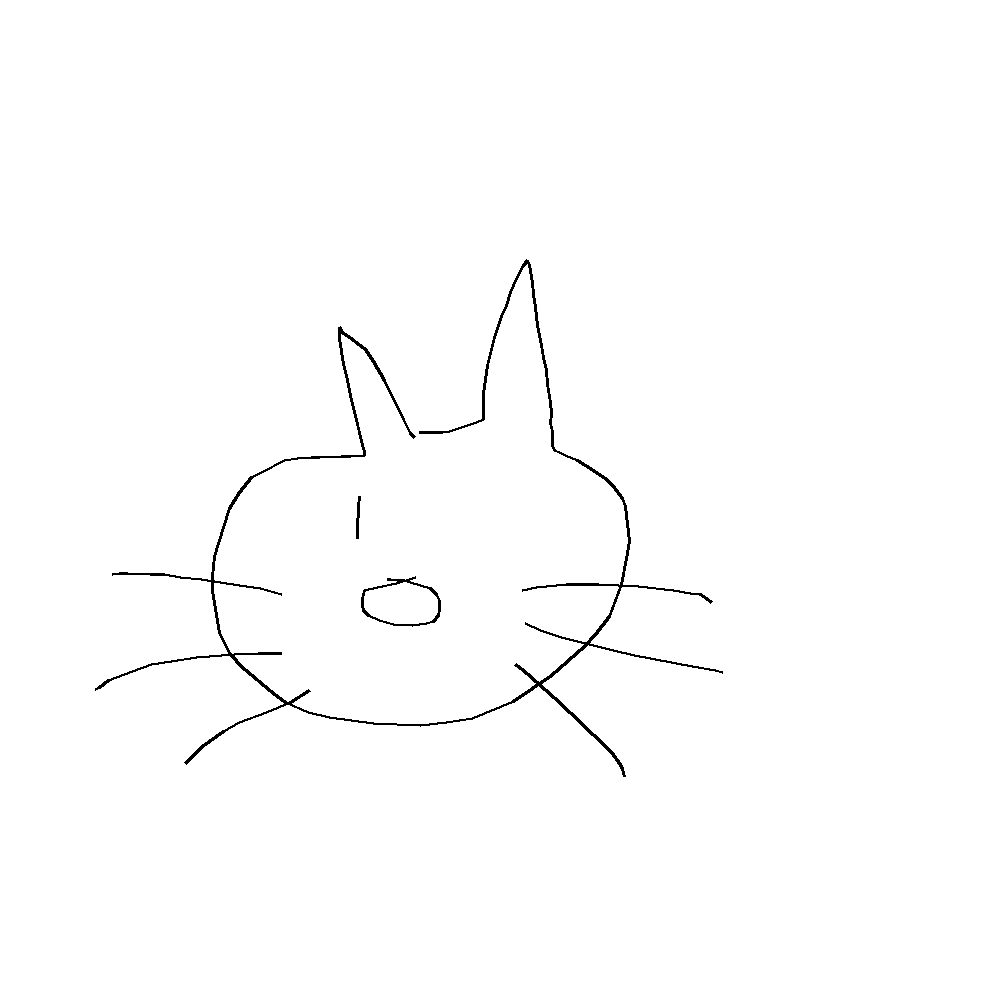
\includegraphics[width=0.5\linewidth, keepaspectratio]{screenshots/my_sample_drawing.png}
    \caption{My Sample Drawing}
    \label{fig: My Sample Drawing}
\end{figure}

Subsequently, the preprocessed drawings were processed through the CoSE model's core functions: encoding strokes into a latent space, predicting the position of the next stroke, computing the latent representation for the upcoming stroke, and reconstructing the predicted stroke on the canvas (see Appendix \ref{appendix: model signatures} for more details). This iterative process allows the CoSE model to generate complex structures based on individual stroke characteristics and their interrelations. 

Finally, I calculated the entropy of the Gaussian mixture model and the Bhattacharyya distance for each stroke in the sample drawing (see Appendix \ref{appendix: calculate_entropy_python} and Appendix \ref{appendix: calculate_bhattacharyya_python} for more details). The resulting arrays of flexibility measures were visualized using line charts (see Figure \ref{fig: Line Charts of Flexibility Measures for My Sample Drawing}, which revealed valuable insights into the evolving creative process. The high entropy values indicated broad exploration, while the Bhattacharyya distances highlighted significant diversity between the next potential strokes. The high correlation between these two measures is visually corroborated by the line chart, which indicates a similar trend of changes. 

\begin{figure}[htbp]
    \centering
    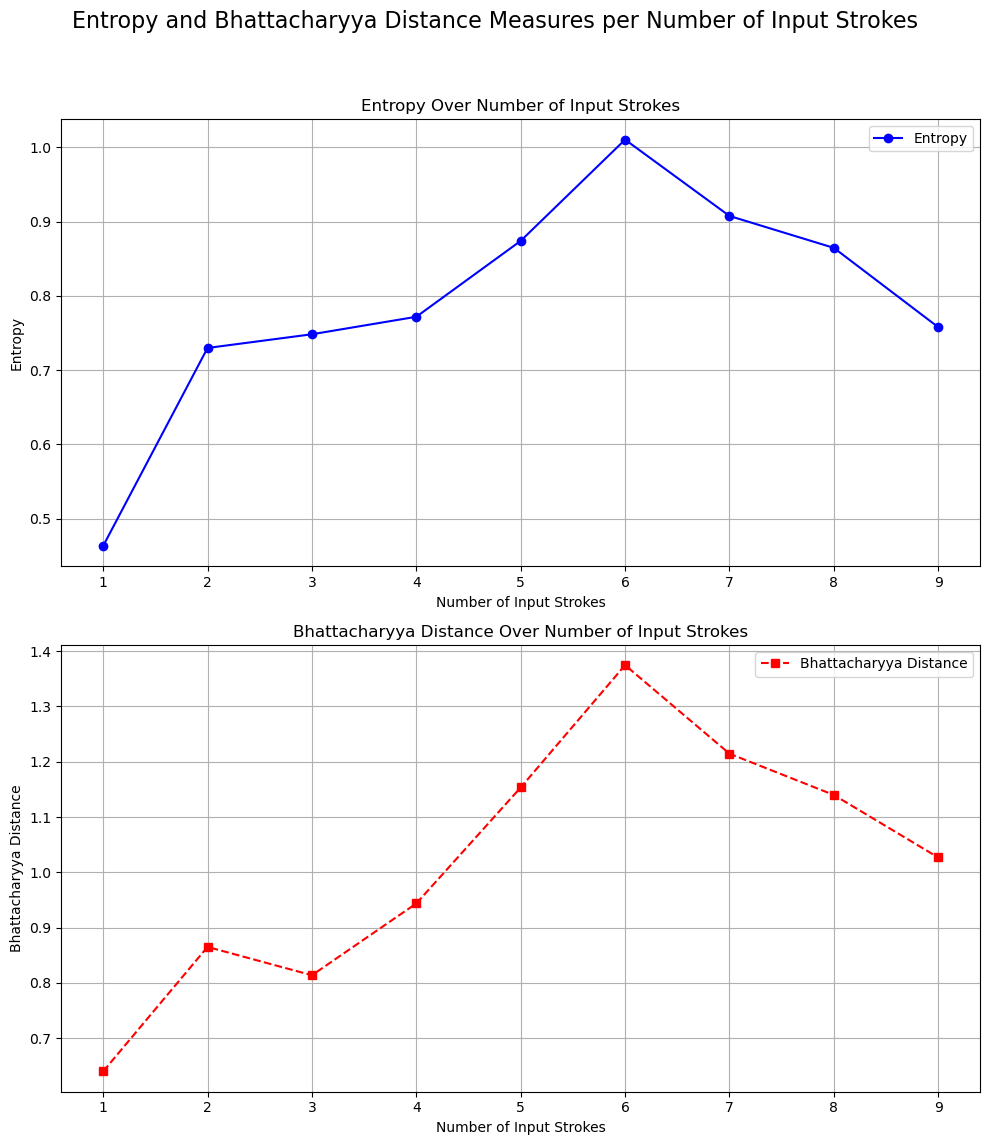
\includegraphics[scale=0.7]{screenshots/Entropy and Bhattacharyya Distance Measures per Number of Input Strokes.png}
    \caption{Line Charts of Flexibility Measures for My Sample Drawing}
    \label{fig: Line Charts of Flexibility Measures for My Sample Drawing}
\end{figure}

However, one thing to notice from the two line charts is that they both do not follow a simple linear decrease in (flexibility) measures, as I hypothesized earlier. This could be due to an outlier effect of my random drawing, which could be overcome by my (relatively) large sample of participants for my experiment. In addition, by tracking changes in flexibility measures starting from a given number of strokes (compared to all strokes), which is the case in incompleteness shape drawing task where a specific number of strokes are already given, the trend may align closer to my hypothesized trend.

Nevertheless, by plotting these metrics, the line charts illustrate not just static values but also the dynamic shift from high to low, effectively mapping out the cognitive journey from open-ended exploration to specific execution. This graphical representation improves understanding by providing a visual narrative of the cognitive shifts occurring as a function of input strokes (number of strokes drawn). It allows for a direct observation of the inflection points where significant changes in creativity metrics occur, offering empirical support to the theoretical framework posited about cognitive flexibility in creative tasks. The time series of these two flexibility measures, therefore, not only validate the use of the CoSE model in capturing the nuances of creative thought processes but also enrich our understanding of how individuals navigate the complex landscape of creativity.

\subsection*{Testing the Calculation of DSI}
I also simulated the process of calculating another measure of flexibility from participants' verbal description of their creative thought processes: DSI. Specifically, I used the sample narrative text from \textcite{johnson_divergent_2022}'s Open Science Framework (OSF) \href{https://osf.io/ath2s/}{repository} (which contains 179 observations) and calculated DSI scores for each verbal description (see my github repository containing \href{https://github.com/cty20010831/UChicago_MA_Thesis_Divergent-Semantic-Integration/blob/bdd32706afb7ba8e72f07b3b10d1eaa9fe8b4331/user_text/DSI_output.csv.csv}{output csv file}). Table \ref{tab: narratives with top and bottom 2 DSI scores}, which shows the narratives with the highest and lowest 2 DSI scores, offers a glimpse into the valid assessment of DSI of participants' narratives. Specifically, the low DSI scores of narratives 3 and 4 are evident given their straightforward and simplistic content. These narratives consist of short, factual sentences with minimal descriptive detail and lack of complex, divergent ideas. By comparison, narratives 1 and 2, which have high DSI scores, exhibit more unique and imaginative elements. These narratives are characterized by rich descriptive language, emotional depth, and the integration of multiple ideas and themes. 

% Table of narratives with top and bottom 2 DSI scores
\begin{longtable}{|p{13cm}|c|}
    \hline
    Narratives & DSI \\ 
    \hline
    His mother woke up, distressed and unsettled. She only had one more stamp left. Had she really sent that many letters already? Her son left for bootcamp only three weeks ago, and the two books of stamps went much faster than the long days she spent without him, wondering what he could possibly be doing. & 0.823803246 \\ 
    \hline
    She had spent her whole life writing this letter. Every little detail she poured her heart into, making sure it was clear and her voice was loud. She stuck in in the envelop, carefully placed the bright red stamp, and sealed it shut. She got in her car, hands trembling, ready to give her life away in this tiny rectangular package. Sending the letter away was sending apart of her away. And send it she did. & 0.822249174 \\
    \hline
    I wrote a letter to my aunt. I went to the post office and bought a stamp. I put the stamp on the letter and gave it to the mailman to send. & 0.735599697 \\
    \hline
    I wrote a letter to my mom. I am going to send it today. I need to find a stamp first. After I find one, I will send it. & 0.734623551 \\
    \hline
    \caption{Narratives with Top and Bottom Two DSI Scores}
    \label{tab: narratives with top and bottom 2 DSI scores}
\end{longtable}

\subsection*{Testing the AuDrA Model}
Finally, I used the pre-trained AuDrA model to simulate the process of assessing the originality of four sample drawings from \textcite{patterson_audra_2023}'s Open Science Framework (OSF) \href{https://osf.io/kqn9v/}{repository} (see Figure \ref{fig: sample_drawing_AuDrA}). In my opinion, the originality ratings (see Table \ref{tab: audra_sample_rating}) on these sample drawings boast a valid assessment of originality. Specifically, the low originality ratings of drawings 2 and 3 are evident given the lack of distinctive or creative features in these drawings, such as simple shapes and repetitive patterns. By comparison, drawings 1 and 4 exhibit more unique and imaginative elements, including complex shapes, innovative patterns, and creative use of space, which are reflected in their higher originality ratings. This suggests that the AuDrA model effectively captures the nuanced aspects of creativity and originality that align with my expectations and previous assessments.

% Table of originality rating on four sample drawings
\begin{table}[htbp]
    \centering
    \begin{tabular}{c c} 
        \hline
        ID & Originality Rating \\ 
        \hline
        1 & 0.502454519 \\ 
        2 & 0.273976982 \\
        3 & 0.25074771 \\
        4 & 0.589645386 \\
        \hline
    \end{tabular}
    \caption{AuDrA Originality Ratings on Four Sample Drawings}
    \label{tab: audra_sample_rating}
\end{table}

% 2*2 grid of four sample drawings for AuDrA assessment
\begin{figure}[]
    \centering
    \begin{minipage}{0.45\textwidth}
        \centering
        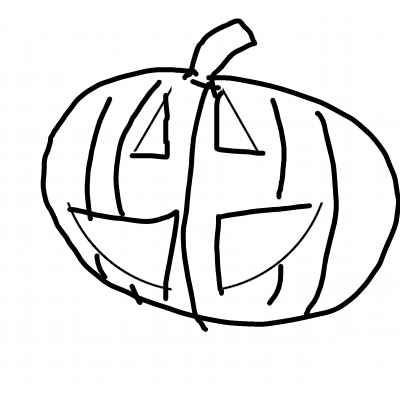
\includegraphics[width=\linewidth]{sample_drawing_AuDrA/example1.jpg}
        \caption*{(a) Sample Drawing 1}
    \end{minipage}\hfill
    \begin{minipage}{0.45\textwidth}
        \centering
        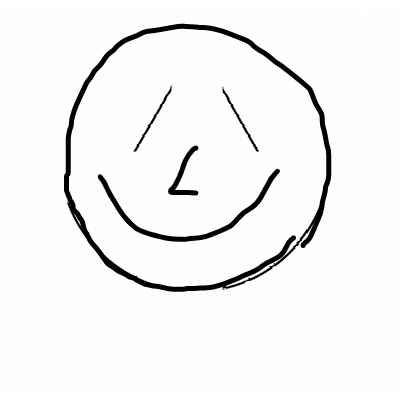
\includegraphics[width=\linewidth]{sample_drawing_AuDrA/example2.jpg}
        \caption*{(b) Sample Drawing 2}
    \end{minipage}
    \vspace{0.5cm}
    \begin{minipage}{0.45\textwidth}
        \centering
        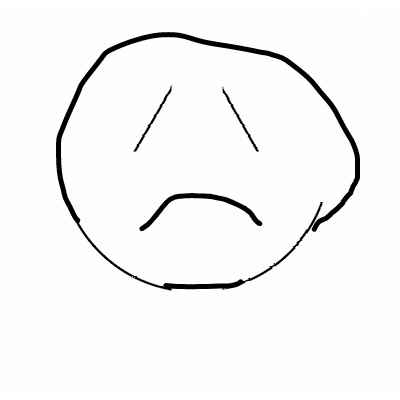
\includegraphics[width=\linewidth]{sample_drawing_AuDrA/example3.jpg}
        \caption*{(c) Sample Drawing 3}
    \end{minipage}\hfill
    \begin{minipage}{0.45\textwidth}
        \centering
        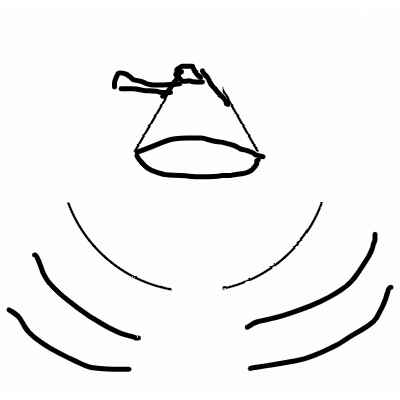
\includegraphics[width=\linewidth]{sample_drawing_AuDrA/example4.jpg}
        \caption*{(d) Sample Drawing 4}
    \end{minipage}
    \caption{Four Sample Drawings for AuDrA Originality Assessment}
    \label{fig: sample_drawing_AuDrA}
\end{figure}


\end{document}
